\section{Landing Platform}
The team members responsible for this part of the project is the Author Daniel, Uffe with mechanical assistance for the prototype and idea generation and Hojat with the electronics.
\subsection{Introduction}
The function of the landing platform is to compensate for the tolerances on the CV guidance system and secure a precise landing. This is needed to establish a good connection with the battery every time. The CV guidance system should be able to operate in a radius of XX cm and a rotation of +- XX degrees.
In this case the idea is to make the platform fit the IRIS drone from 3DR. Though it would be preferred if the system could also be used with other UAS or easily modified to do so.
\subsection{Idea generation}
The team came up with two general ideas for centring and alignment of the drone both using the IRIS's existing legs.
\subsubsection{Connector pods}
Common for both ideas is that there has to be four connector pods on the UAS. The function of these pods is to secure a stable connection of all four connections. One problem could be that the UAS will balance on three pods due to small tolerance problems. This was compensated by making the pods soft. This way they will deflect under the load of the UAS. This will secure all four has connection.
Another challenge  was to mount them easily without modifying the drone to much if at all. This was solved by using the RIS system under each arm on the drone to make a quick lock with two bolts.
\begin{center}
	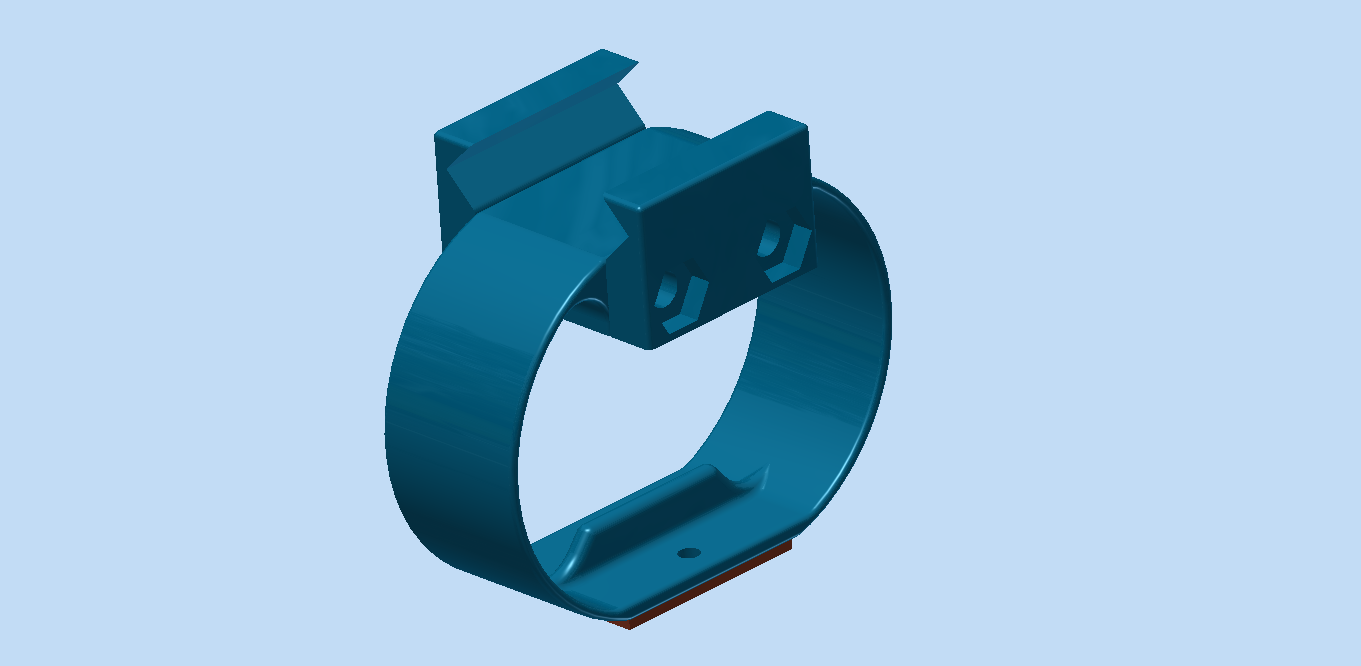
\includegraphics[width=0.8\textwidth]{imgs/connectorpod}
\end{center}
\subsubsection{Landing platform - Idea 1}
The first idea was a negative platform that would have four cone shaped holes, one for each leg. The holes will catch the legs and guide the aircraft in place. Under the body of the UAS there would be a hole in the platform to allow for a camera to see the aircraft on the sky.
\begin{center}
	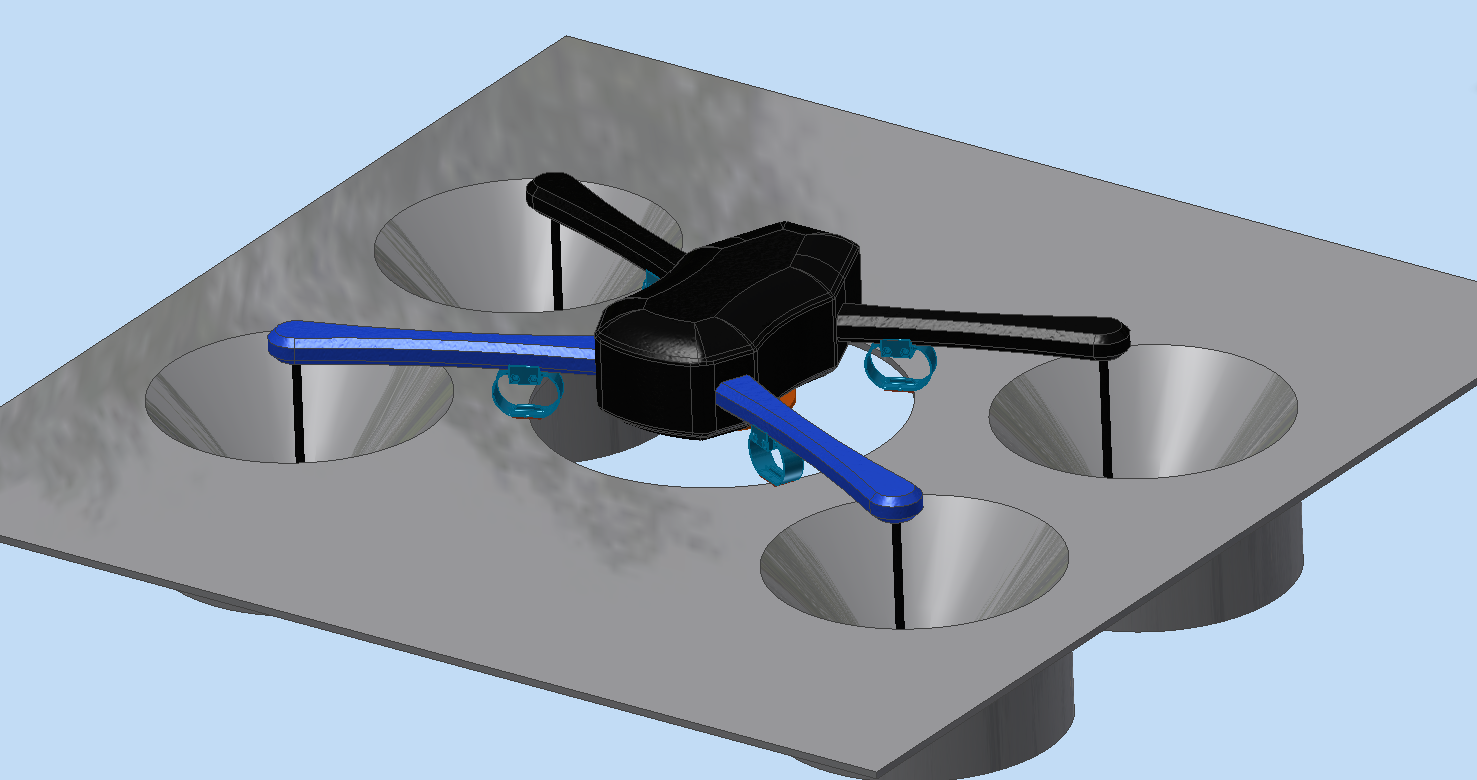
\includegraphics[width=0.8\textwidth]{imgs/mockup_idea_2}
\end{center}
\begin{center}
	\begin{minipage}[t]{0.45\textwidth}
		\begin{flushleft}
			\emph{Advantages}\\
			Few parts (connectors and marker) added to the UAV\\
			Completely locked position (x, y, z) when landed
		\end{flushleft}
	\end{minipage}
	\begin{minipage}[t]{0.45\textwidth}
		\begin{flushleft}
			\emph{Disadvantages}\\
			Ground effect on rotors\\
			Complicated construction \\
			4 individual landing spots to hit\\
			Must land rather precise as rotation plays a big role
		\end{flushleft}
	\end{minipage}
\end{center}

\subsubsection{Landing platform - Idea 2}
The second idea was a positive platform, that would have one big cone with a flat top(volcano shape). On the aircraft's leg there would be mounted a ring of a flexible and light material to guide the aircraft in place. Under the body of the UAS there would be a hole in the platform to allow for a camera to see the aircraft on the sky.

\begin{center}
	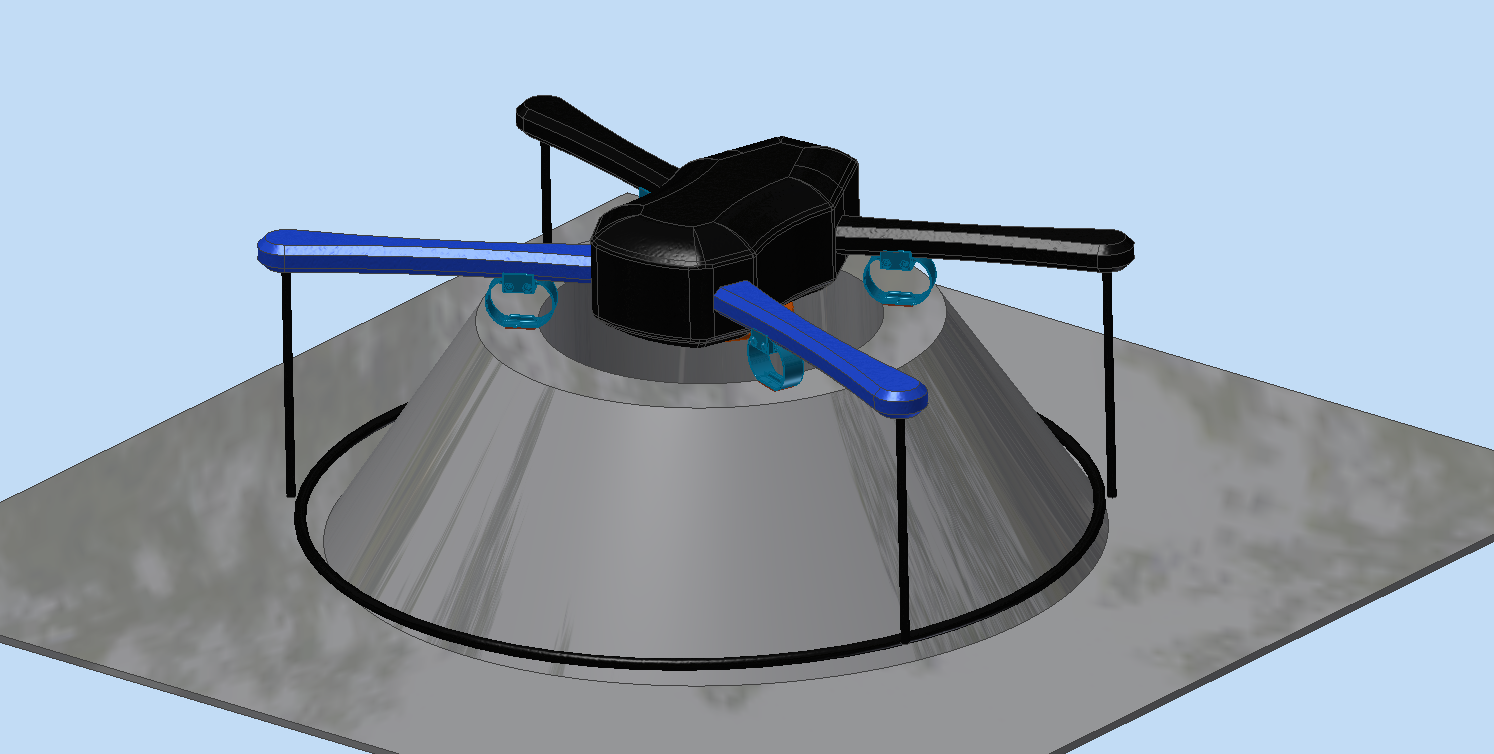
\includegraphics[width=0.8\textwidth]{imgs/mockup_idea_1}
\end{center}
\begin{center}
	\begin{minipage}[t]{0.45\textwidth}
		\begin{flushleft}
			\emph{Advantages}\\
			None or very little ground effect\\
			Simple construction\\
			One landing spot to hit with the UAV
			Allows for the UAV to rotate rather much without connection problems
		\end{flushleft}
	\end{minipage}
	\begin{minipage}[t]{0.45\textwidth}
		\begin{flushleft}
			\emph{Disadvantages}\\
			Adds more weight to the UAV
		\end{flushleft}
	\end{minipage}
\end{center}

As the final idea we chose idea 2. This seems to be the most tolerant idea for the CV. and it's very simple in construction compared to the little extra weight added to the UAS. Also the effect on the UAS's stability is much less due to the aerodynamic of the cone compared to the flat plate on the other design which will get fairly close to the rotors compared to here.

\subsection{Testing}
First the general concept of the idea was tested with an early prototype of the platform chosen. This was also done to see what the smallest angle on the edges could be without tipping the drone instead of sliding it in place.

\begin{center}
	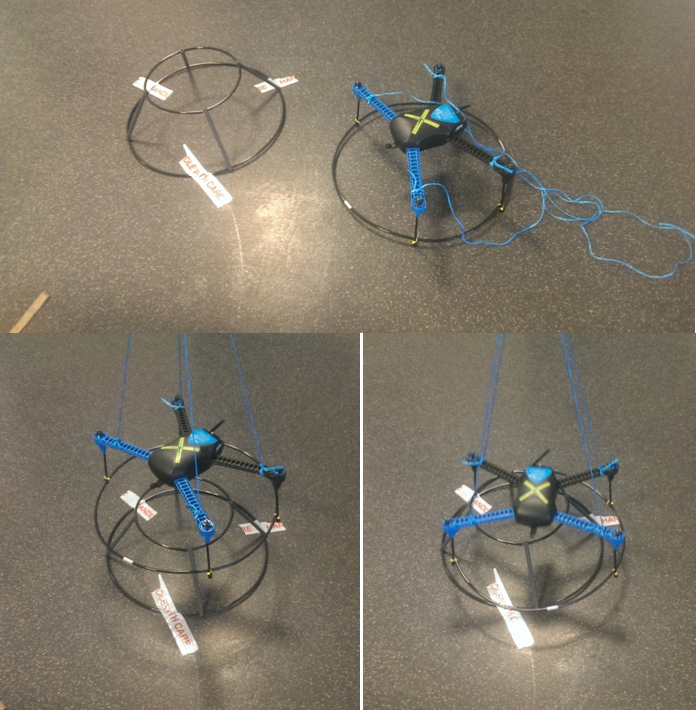
\includegraphics[width=0.8\textwidth]{imgs/prototype1_test}
\end{center}

We found that the concept works. The drone slides in place instead of tilting over. The angle should not be any bigger than the one the platform prototype had at first so this was the angle we chose.

We also made four prototypes of the connector pods on a 3D printer.

\Huge{\textbf{XX Billede af connector pods}}

\normalsize
The pods were tested to see if the connection was good. Each connector pod on the drone was connected to one of the following: ground, cell 1, cell 1-2 and cell 1-3. On the platform the four connector pads were connected to 4 LED's showing contact and the connection with each cell has been established.

\Huge{\textbf{XX Billede af test med LED'er på endelig prototype}}

\normalsize
As the picture above shows the landing pad was connected to all four connector pods with success. However the connection would be more stable if the connector pods were softer. This could be done with another plastic than the rather stiff PLA or with a softener added.
\subsection{Final design}

weight!


\subsection{Further development}
The landing platform developed in this project has no environmental protection of the connector pads and UAS when docked. This project's main focus was to land and dock the aircraft ready to charge. For further development the concept developed in this report will have to be put in a box of some kind that will protect the UAS and electronics of the platform in bad weather.

This could be a bigger shed-like construction that will act as a windbreak to make landing easier. The shed would then have to have a roof that can open itself. Or simply just a small box that opens a lid and expose the platform in good weather and maybe even lift the landing pad free of the walls to eliminate aerodynamic problems from the box's walls

\begin{center}
	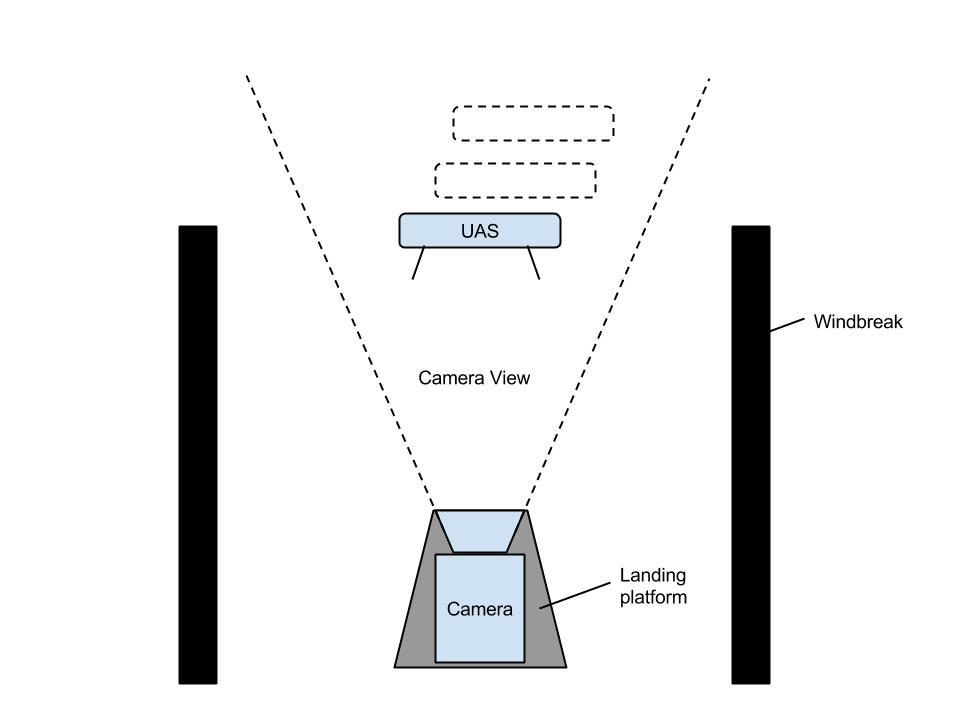
\includegraphics[width=0.8\textwidth]{imgs/landing_platform}
\end{center}

\subsection{Part conclusion}